\title{Identifying Breast Cancer Gene Signatures with Feature Selection}
\author{
        \textsc{Gustavo Empinotti}
            \qquad
        \textsc{Susan Tu}
            \qquad
        \textsc{Raf Mertens}
        \mbox{}\\ %
        \\
        CS229\\
        \mbox{}\\ %
        \normalsize
            \texttt{gustavoe}
        \textbar{}
            \texttt{susanctu}
        \textbar{}
            \texttt{rafm}
        \normalsize
            \texttt{@stanford.edu}
}
\date{\today}
\documentclass[11pt]{article}
%\documentclass{acmconf}
\usepackage[pdftex]{graphicx}
\usepackage[paper=a4paper,dvips,top=1.5cm,left=1.5cm,right=1.5cm,
    foot=1cm,bottom=1.5cm]{geometry}
%----------------------------------------------------------
\begin{document}

\maketitle

\begin{abstract}
Statistical or machine learning methods have been used to find cancer gene signatures intended to predict survival or to classify patient prognosis as good/poor. However, a recent paper suggests that random gene subsets perform as well or better than 47 published gene signatures obtained through statistical methods, perhaps because cancer disrupts expression of many genes not directly related to cancer \cite{venet}. In this paper, we use different feature selection methods in an attempt to find a small set of genes that distinguishes normal breast tissue from malignant tumor tissue. We plan to compare the predictive power of our selected genes to that of random gene subsets, gene subsets that should be unrelated to cancer, and previously published gene signatures.
\end{abstract}

\section{Introduction}

\section{Methods}


\section{Results \& Discussion}

\subsection{Forward Selection}
The most straightforward method for feature selection is forward selection. We ranked the genes by Chi2 statistic. This statistic measures the dependence between random variables, so we select the features that are least likely to be independent of class. One downside of this method is that if 2 relevant features are (nearly) identical, we select both even though really only one of the two gives us new information. We clearly observe this phenomenon. \\\\
For example selecting the 50 most relevant features using all our data results in the following list of genes:\\\\
'HLA-DRB5' 'HLA-DRB6' 'HLA-E' 'HLA-F' 'HLA-G' 'HLCS' 'HMG2L1' 'HMGCS2'
 'HMHB1' 'HMOX2' 'HMP19' 'HMX2' 'HN1' 'HN1L' 'HNMT' 'HNRNPC' 'HNRNPU'
 'HNRPCL1' 'HOXA6' 'HOXA7' 'HOXA9' 'HOXB1' 'HOXB2' 'HOXB3' 'HOXB6' 'HOXC10'
 'HOXC11' 'HOXC12' 'HOXC13' 'HOXC4' 'LOC92345' 'SLC7A13' 'SLC9A10'
 'SLC9A3R1' 'SLC9A3R2' 'SLC9A4' 'SLC9A7' 'SLC9A8' 'SLC9A9' 'SLCO1C1'
 'SLFN12' 'SLFN13' 'SLFN5' 'SLFNL1' 'SLIC1' 'SLIT2' 'SLIT3' 'SLITRK3'
 'SLITRK4' 'SLK'
 
Many of which are obviously related (e.g. HOXC11, HOXC12, ...).\\\\
To measure the prediction power of our model we used 4-fold cross validation. To do this, we only use the training data to do feature selection, since we otherwise encode information about the test data into our model. Using a SVM we get the following results averaged over the 4 fold cross validation parts:\\\\
average accuracy: 0.984998675\\
average precision: 0.985778285\\
average recall 0.998120301\\\\
We can compare this to using an SVM with all features, again using 4 fold cross validation:\\\\
average accuracy 0.911570558\\
average precision: 0.909611142\\
average recall: 1.0\\
\subsection{Backwards Selection}
\subsection{Logistic Regression}

\begin{figure}[h!]
  \centering
    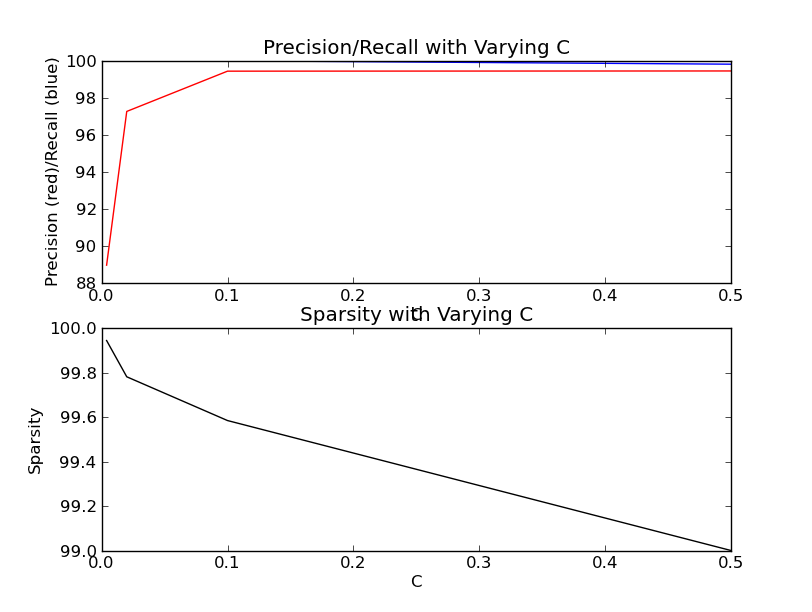
\includegraphics[scale=0.5]{sparselog.png}
  \caption{Results of logistic regression with regularization.}
\label{fig:sparselog}
\end{figure}
%will not be including huge lists of genes in the final doc, but since we haven't evaluated these lists yet, just putting them here as what-we-have-so-far
The precision and recall for a logistic regression with no regularization were 0.9945255474452555 and 0.996267825311943. As can be seen in Figure \ref{fig:sparselog}, C=0.01 provides reasonable precision/recall while still providing a reasonably small number of selected features. The genes selected when C=0.01 are $[$'ADAMDEC1', 'ANGPTL7', 'AREG', 'ASPN', 'C20orf103', 'C20orf54', 'CA4', 'CAMP', 'CCL11', 'COL10A1', 'COL11A1', 'COL1A1', 'COMP', 'CST1', 'CTHRC1', 'CXCL11', 'CXCL2', 'DLK1', 'FABP7', 'FAM111B', 'FAM19A4', 'FGB', 'FGFBP1', 'FHL1', 'FLJ35773', 'FLJ45557', 'GDF10', 'GGTA1', 'GJB2', 'GLRA3', 'GPC3', 'GPR84', 'GSTA2', 'HMGCLL1', 'IGFBP1', 'IGSF10', 'INHBA', 'KIAA1576', 'KIF2C', 'KLRC3', 'LOC152573', 'LOC55908', 'LRRC3B', 'MAOA', 'MKI67', 'MMP10', 'MMP11', 'MMP13', 'MMP3', 'MMP9', 'MUCL1', 'MYEOV', 'MYPN', 'NLGN1', 'NR0B1', 'NUF2', 'OCA2', 'PCK1', 'PCOLCE2', 'PPAPDC1A', 'PPEF1', 'PTPRZ1', 'PTX3', 'RBP4', 'S100B', 'SFRP2', 'SPINK5', 'SSTR1', 'SYT13', 'TFPI2', 'TSLP', 'VCX2', 'WISP1', 'ZBED2'$]$.
\begin{thebibliography}{9}

\bibitem{venet}
  David Venet, Jacques E. Dumont, Vincent Detours
  Most Random Gene Expression Signatures are Significantly Associated with Breast Cancer Outcome
\end{thebibliography}
\end{document}
